\section{Issues and solutions}
The following sections represent challenges that the team encountered, and how these challenges were met.

\subsection{Unplanned absence}
One of the team members, Lars Erik, had to make a sudden trip abroad due to
death in the family. He was away from the team for a total for 12 days. Prior
to departure the team divided the tasks with a lighter workload assigned to Lars
Erik, as described in the risk analysis. Even with the redistributed workload
the team and Lars Erik in particular found the distance and time difference to
be a bigger problem than expected. Some work was left undone and had to be
picked up at the end of the sprint or pushed to the next sprint. The team
learned that the impact of such leaves of absence should probably be
overestimated rather than underestimated in the eventuality of another event.

\subsection{Workplace issues}
The team had booked meeting rooms three times a week in NTNUs IT building to host the work sessions. Unfortunately, the building was under renovation the for the entire duration of the project. Booking other rooms that fit the teams needs so late in the semester proved to be difficult. This issue lead to periods where the team were disturbed a lot by the construction, which in turn lead to team members growing tired and being a bit more on edge than usual. To counter this, the team instated a cake policy. Every Wednesday, a team member would bring something good to eat as well as making sure that the other team members took regular breaks from the work. This helped ease the tension of the work sessions.

\begin{comment}
\subsection{Excessive discussion}
The team has seen that much time is being spent discussing a lot. The discussion was of importance, but it drained too much of the time. To solve this, it was decided that there should be set a certain amount of time for the discussions. Should the discussions last longer than the time set, the project leader's task was to focus on ending the discussions, and instead perform a democratic vote based on the arguments that were presented. 
\end{comment}


\subsection{Traveling to China}
In the beginning of April the entire team left for a school trip to China. This meant that the team would be unavailable for at total of 17 days, including weekends and the Easter holidays. The team decided to not expect that any work would be done during the trip. To make up for the absence, the team increased the number of work hours by 30 extra hours per week. As a result of this, the team would work the same amount of hours as if we never took the trip to China.

\subsection{Changing roles}
\label{sec:unbalancedWorkload}
During sprint five, the team evaluated whether the use of the team's available resources actually were fully exploited. It was acknowledged that our (now former) Scrum master, Per Øyvind, had the best control of the development environment, which in turn lead to that the workload he got due to his position as Scrum master and his level of expertise, was too great. The team therefore decided that Lars Erik, which previously was our deputy project leader, was the best fit to be the new Scrum master.

It was also discussed whether the position ''Project leader'' actually was necessary, as it conflicted with one of the principles in Scrum. \todo{The team decided that we in fact thought the position was necessary, as the project leader and Scrum master simply distributed the Scrum master's traditional tasks between them.} The main difference would be that the project leader would handle the administrative tasks, such as room booking for meetings and work sessions, and handle customer relations, while the Scrum master would handle the project administrative tasks, such as moderating the Scrum meetings, adding tasks to the backlog and Yodiz, and generate burn down charts.


\subsection{Improper use of Yodiz}
\label{sec:improperScrum}
As mentioned in section~\ref{sec:scrumtool}, the team used a lot of time on
deciding on which Scrum tool to use for the project management. Although our
choice fell on Yodiz, the team was in lack of any previous experience with the
tool, and despite the team's efforts to get acquainted with the tool, a
misunderstanding arose and was not discovered until the end of the second
sprint.

The misunderstanding, displayed in figure~\ref{fig:wrongUse}, was that the team
assumed one could add multiple individuals as responsible on a particular task,
while Yodiz' functionality only assigned the time spent to the individual that
either created the task or was assigned as owner of the task.

As a result, it appeared as if only singular individuals performed the tasks,
even though the entire team in reality was participating, which was also
reflected in the burn down charts and the generated Gantt diagram. 

To sort out this issue, the team went through old meeting reports and time sheets
to figure out which members of the team that had actually participated on the
particular task, and added new tasks and the time spent to the members that at
the time had not recorded this information.%, as shown in figure~\ref{fig:addsTasks}.

This issue was unfortunate, but not insurmountable, and also not a critical
issue for the overall progress of the project.

\begin{figure}[H]
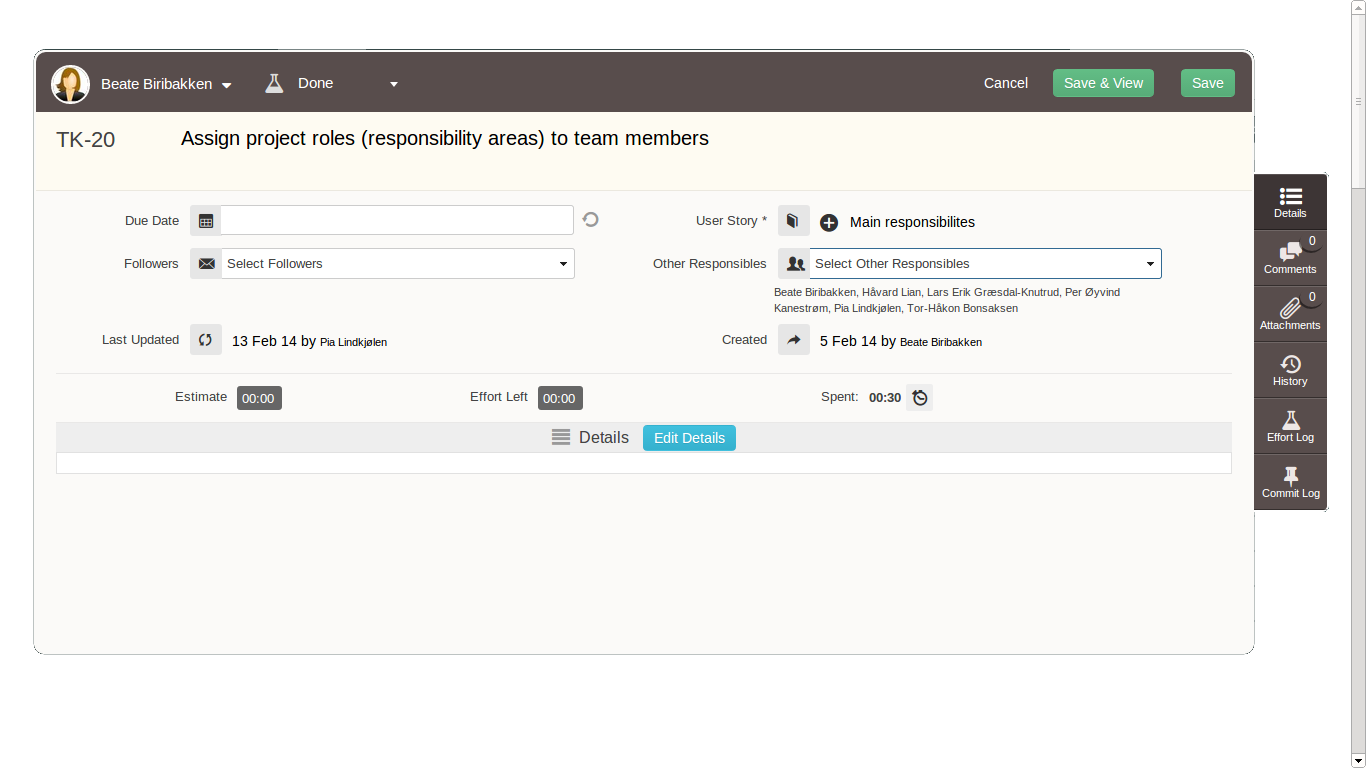
\includegraphics[width=\textwidth, clip, trim=1cm 2cm 4cm 1cm]{ch/retrospect/fig/wrongUse.png}
\caption{Example screenshot to illustrate improper use of Yodiz}
\label{fig:wrongUse}
\end{figure}